\begin{multicols}{3}[\section{WiMAX}]

\rhead{Alexander Härtel, Elias Holz}
\lfoot{08.05.2016}

\newrefsegment

\begin{tabular}{p{2,1 cm}p{2.7 cm}}
\textbf{Steckbrief}& \\
\end{tabular}
\rowcolors{1}{\topicolor!20}{}
\begin{tabular}{p{2,1 cm}p{2.7 cm}}
      Einsatz seit & 2004\\
      Standards & IEEE 802.16d-2004, IEEE 802.16e-2005, IEEE 802.16m\\
      Frequenzbereich  & \SI{2}{\giga\hertz} - \SI{11}{\giga\hertz}\\
      Bandbreite & \SI{1,5}{\mega\hertz} - \SI{20}{\mega\hertz}\\
      Datenrate & bis zu \SI{1}{Gbit/s}\\
      Topologie & Sterntopologie oder Meshed Network\\
      Verbreitung & Weltweit\\
      Reichweite & bis zu \SI{50}{\kilo\metre}\\
      Modulation & 64QAM, 16QAM, QPSK, BPSK\\
      Multiplexverfahren & OFDM265, SOFDM, OFDMA, MIMO\\
      Verschlüsselung & AES\\
\end{tabular}
\par
%Source http://www.fh-bingen.de/fileadmin/user_upload/Lehrende/Kilsch_Dieter/internet/projekte/TedoSchStiUnits.pdf -> Seite 9 findet ihr alle verwendbaren Einheiten, wie:
%\SI{Zahl}{\mega\hertz} oder \SI{Zahl}{\mili\metre}
%Ich weiß ehrlich gesagt nicht welche Einheiten ihr im Text genau braucht, aber in dem Dokument und mit obigen Beispiel sollte es umsetzbar ein.
\subsection*{Überblick}
\begin{wrapfigure}{r}{0.4\linewidth}
  \vspace{-20pt}
  \begin{center}
  	\hspace{-20pt}
    
\includegraphics[width=0.7\linewidth]{Kapitel/WiMAX/Grafiken/wmx_logo.jpg}
  \end{center}
  \vspace{-15pt}
\end{wrapfigure}

\textit{\textbf{WiMAX}} (\textit{\textbf{W}orldwide \textbf{I}nteroperability for \textbf{M}icrowave \textbf{A}ccess}) ist eine \enquote{Highspeed Funktechnologie für breitbandige, bidirektionale Hochgeschwindigkeitsübertragung im Zugangsnetz}.~\cite{wmx.1}

\textit{WiMAX}  ist dabei ideal für den Aufbau von \textbf{MAN}'s (\textbf{M}etropolitan \textbf{A}rea \textbf{N}etwork) mit stationären und mobilen Endgeräten geeignet, daher auch der Beiname \enquote{Hiper-MAN}. \textit{WiMAX} wird durch einige Profile des \textit{\textbf{IEEE}} (\textit{\textbf{I}nstitute of \textbf{E}lectrical and \textbf{E}lectronics \textbf{E}ngineers}) 802.16 Standards definiert und wurde parallel zum \textit{IEEE} 802.11 \textbf{WLAN}-Standard (\textbf{W}ireless \textbf{L}ocal \textbf{A}rea \textbf{N}etwork) entwickelt, allerdings mit dem Ziel, eine Alternative zu \textbf{DSL} (\textbf{D}igital \textbf{S}ubscriber \textbf{L}ine) zu bieten.~\cite{wmx.2}

Im \textit{\textbf{OSI}}-Modell (\textbf{O}pen \textbf{S}ystems \textbf{I}nterconnection) spezifiziert es die untersten beiden Schichten (Physical Layer und Medium Access Control Layer). Aufgrund eines Frequenzbandes von 2 - 11 GHz und dem fehlenden Bedarf einer leitungsgebundenen Infrastruktur ist der Standard weltweit einsetzbar und vor allem in Regionen ohne DSL oder Kabelinternet interessant.~\cite{wmx.4}


\subsection*{Technische Erläuterung}
\subsubsection*{Überblick}
\textit{WiMAX} setzt sich im Wesentlichen aus drei spezifizierten Standards zusammen:
\begin{itemize}
	\item \textbf{\textit{IEEE} 802.16d-2004:} auch Fixed \textit{WiMAX}: für statische Verbindungen ohne Handover (= Endgerät wechselt während einer Datenverbindung ohne Unterbrechung dieser Verbindung von einer Funkzelle in eine andere~\cite{wmx.10}) für Sicht- und Nichtsichtverbindungen im Frequenzbereich von 2 - 11 GHz und Bandbreiten bis zu 20 GHz.
	\item \textbf{\textit{IEEE} 802.16e-2005:} auch Mobile \textit{WiMAX}: erlaubt nun Handover und zeichnet sich durch einen erhöhten Datendurchsatz  und eine verbesserte Signalstabilität aus. Nutzt einen Frequenzbereich von 0,7 - 6 GHz bei bis zu 15 MBit/s.
	\item \textbf{\textit{IEEE} 802.16m:} auch \textit{WiMAX} 2: Highspeed-Übertragung bis zu 1 GBit/s bei einer Reichweite bis zu 30 km.
\end{itemize}
In städtischer Umgebung hat \textit{WiMAX} eine Reichweite von 2 - 5 km, wobei die zur Verfügung stehende Datenrate auf die Teilnehmer aufgeteilt wird.~\cite{wmx.4}

\subsubsection*{Architektur}
Der 802.16 Standard sieht ein Netz bestehend aus Basis- und Subscriberstationen vor (kurz: \textbf{BS} und \textbf{SS}), wobei die Subscriberstationen die Sende- und Empfangsgeräte beim Kunden darstellen, daher auch die Bezeichnung \textit{WiMAX}-Modem. Ein \textit{WiMAX}-Modem besteht dabei neben dem eigentlichen Funkmodem aus einem Router und einer kleinen \textbf{VoIP}-Anlage (\textbf{V}oice \textbf{o}ver \textbf{I}nternet \textbf{P}rotocol).

Ein \textit{WiMAX}-Netz wird in der Regel als Sterntopologie zwischen den BS und den SS aufgebaut, da die Basisstation nun die Konfiguration und Verwaltung zentral übernehmen kann. Dadurch können nicht nur Kosten bei den SS durch kleineren Funktionsumfang gespart werden, sondern auch die Quality of Service gewährleistet werden. Neben dieser Sterntopologie ist aber auch der Aufbau eines Meshed Networks zwischen mehreren SS möglich.

Als Funkantennen kommen wie in Abbildung \ref{fig:bild.antenne} zu sehen bei den SS meist klassische Haus- oder Wandantennen zum Einsatz (auch Vertikalantennen möglich), oberhalb einer Sendefrequenz von 10 GHz bietet sich aber auch der Einsatz von Parabolantennen an, wodurch bei Sichtverbindung hohe Übertragungsraten ermöglicht werden.~\cite{wmx.2}

\begin{Figure}
	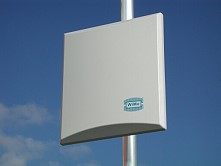
\includegraphics[width=\linewidth]{Kapitel/WiMAX/Grafiken/Antenne.jpg}
	\captionof{figure}{Eine handelsübliche WiMAX-Antenne ~\cite{wmx.14}}
	\label{fig:bild.antenne}
\end{Figure}

\subsubsection*{Kommunikation}
Die Kommunikation geschieht in \textit{WiMAX} über die 4 Schichten: Physical Layer, Transmission Layer (gleichbedeutend mit dem Data Link Layer des \textit{OSI}-Modells), MAC-Layer und Convergence Layer. Auf jeder Schicht stellt \textit{WiMAX} dabei mehrere Interfaces und Protokolle für die Kommunikation zur Verfügung, wie zum Beispiel Ethernet, \textbf{TDM} (\textbf{T}ime \textbf{D}ivision \textbf{M}ultiplexing), \textbf{ATM} (\textbf{A}synchronous \textbf{T}ransfer \textbf{M}ode), \textbf{IP} (\textbf{I}nternet \textbf{P}rotocol) oder \textbf{VLAN} (\textbf{V}irtual \textbf{L}ocal \textbf{A}rea \textbf{N}etwork). Nennenswert ist noch der Einsatz von \textbf{IPsec} (\textbf{I}nternet \textbf{P}rotocol \textbf{Sec}urity) im Kernnetz, das durch Verschlüsselung jedes IP-Pakets  die Sicherheit erhöhen soll.~\cite{wmx.11}
Die Funkverbindung ist zudem \textbf{AES}-verschlüsselt (\textbf{A}dvanced \textbf{E}ncryption \textbf{S}tandard), wobei sich die Gegenstellen automatisch konfigurieren und in regelmäßigen Abständen den Schlüssel neu austauschen.~\cite{wmx.8}

\subsubsection*{Übertragung und Modulation}
Ein wesentlicher Aspekt bei \textit{WiMAX} ist die Gewährleistung der Quality of Service. Dies wird im Wesentlichen erreicht durch:
\begin{itemize}
	\item Dynamische Frequenzanpassung (DFS): Suchen eines Frequenzkanals bei Verbindungsaufbau, der noch nicht belegt ist. Hat direkten Einfluss auf die Sendeleisung und wird ebenfalls in WLAN-Netzen eingesetzt.~\cite{wmx.13}
	\item Regelung der Ausgangsleistung (APC)
	\item Kanalkodierung nach dem Vorwärtsfehlerkorrekturverfahren mit der Reed-Solomon Kodierung zur Senkung der Bitfehlrate
	\item Anforderung von Empfangsbestätigung (ARQ)
	\item Verbindungsorientierung auf Sicherungsschicht
\end{itemize}
Hinzu kommen weitere Techniken und Multiplexverfahren zur Verbesserung des Signalempfangs. Zu nennen sind hier das Orthogonale-Frequenz-Multiplex-Verfahren, welches durch orthogonal stehende Trägerfrequenzen eine gegenseitige Beeinflussung reduziert und das MIMO-Verfahren, welches mehrere Antennen für das Senden und Empfangen einsetzt und so die Kapazität des Netzes deutlich erhöht.~\cite{wmx.12}

Moduliert wird das Signal dabei mit \textbf{QPSK} (\textbf{Q}uadrature \textbf{P}hase-\textbf{S}hift \textbf{K}eying), \textbf{BPSK} (\textbf{B}inary \textbf{P}hase-\textbf{S}hift \textbf{K}eying), \textbf{16QAM} (aus \textbf{16}-Symbolen bestehende \textbf{Q}uadrature \textbf{A}mplitude \textbf{M}odulation) und 64QAM.~\cite{wmx.2}

\subsubsection*{Übertragungsgeschwindigkeit, Reichweite und Frequenzband}
In der Theorie sind bis zu 50 km Reichweite möglich, in der Praxis ist die Reichweite jedoch auf wenige km beschränkt, da mit zunehmenden Radius die Übertragungsgeschwindigkeit stark abnimmt. Dabei sind Kanalbandbreiten von 1,25 - 20 Mhz bei einer Geschwindigkeit von bis zu 75 MBit/s bei stationärem WiMAX, bzw. ca. 10 MBit/s bei mobilem WiMAX möglich (aufgeteilt in Up- und Downlink).~\cite{wmx.1}
Abbildung \ref{fig:bild.frequency} bietet eine Übersicht über weltweit eingesetzte Frequenzbereiche.
\begin{Figure}
	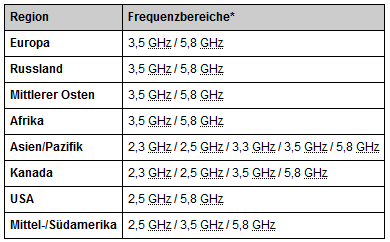
\includegraphics[width=\linewidth]{Kapitel/WiMAX/Grafiken/Frequenztabelle.png}
	\captionof{figure}{Übersicht der eingesetzten Frequenzbereiche ~\cite{wmx.2}}
	\label{fig:bild.frequency}
\end{Figure}

\end{multicols}
\newpage
\section*{Historische Entwicklung}
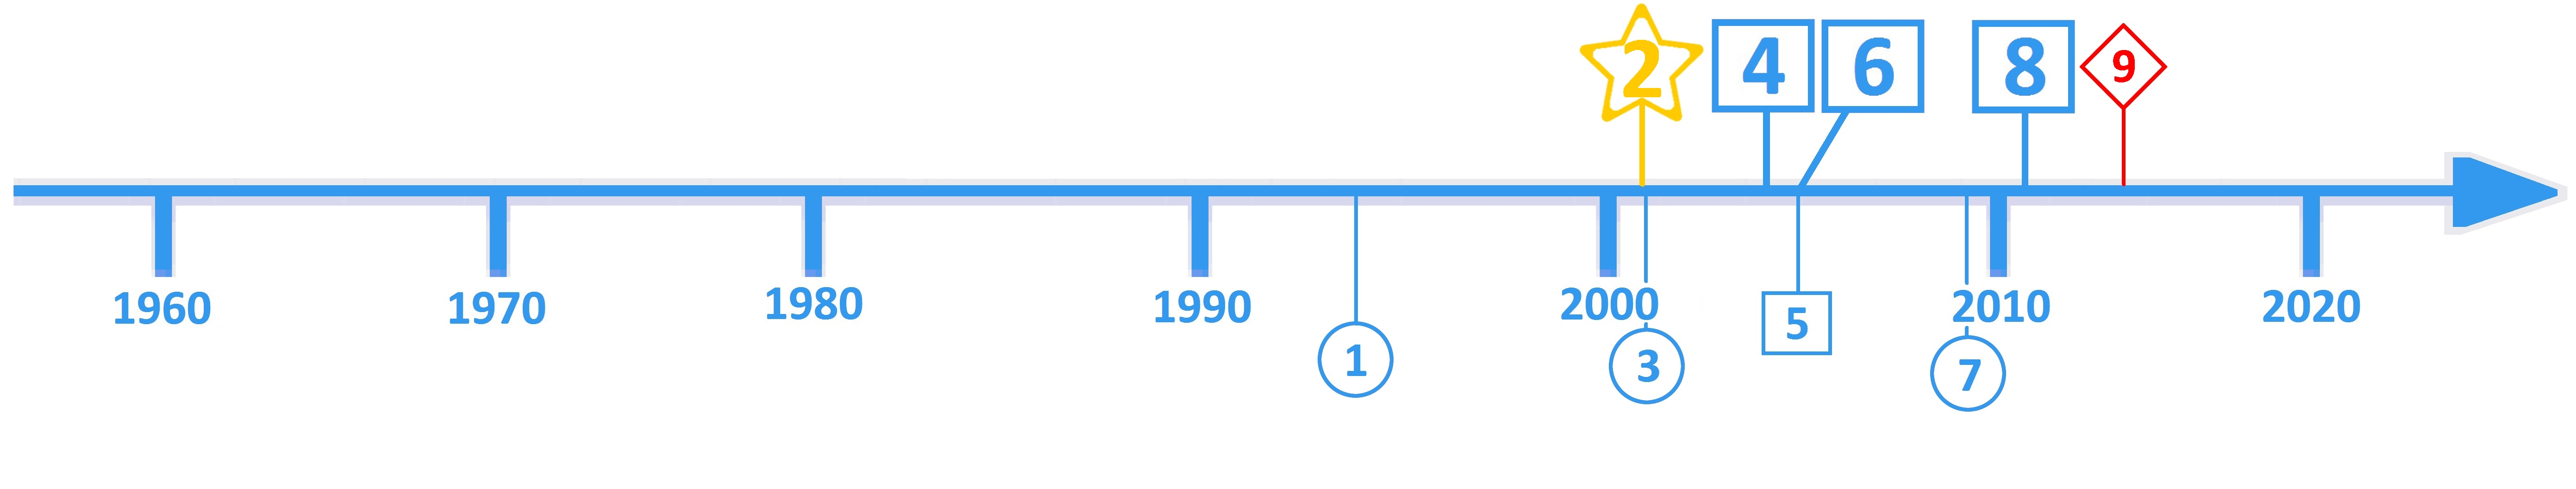
\includegraphics[width=\textwidth]{Kapitel/WiMAX/Grafiken/Zeitstrahl}
\par
\noindent
\rowcolors{2}{}{\topicolor!20}
\begin{tabular}{p{0.5 cm}p{1.5 cm}p{15.55 cm}}
	Nr. & Datum & Entwicklungsschritte~\cite{wmx.2}\\
	1 & 1994 & Standardisierung des ersten DSL Standards \textbf{HDSL} (\textbf{H}igh Data Rate \textbf{D}igital \textbf{S}ubscriber \textbf{L}ine) für kabelgebundenes Internet.~\cite{wmx.5}\\
	2 & 2001 & Beginn der Entwicklung einer Reihe von kabellosen Internet-Standards durch \textit{IEEE} 802.16\\
	3 & 2001 & Aufbau des ersten UMTS-Netzes in Großbritannien (als Konkurrenz zu WiMAX).~\cite{wmx.6}\\
	4 & 2004 & Erste \textit{WiMAX}-Spezifikation \textit{IEEE} 802.16d auf Basis des 802.16 Standards als Funkübertragungssystem für stationäre Verbindungen\\
	5 & 2005 & Lizenzvergabe und Aufbau erster \textit{WiMAX}-Netze\\
	6 & 2005 & Spezifikation von Mobile \textit{WiMAX} mit dem \textit{IEEE} 802.16e Standard\\
	7 & 2009 & Inbetriebnahme erster LTE-Netze als Highspeed-Zugangsnetze (und somit Konkurrenz zu \textit{WiMAX} 2).~\cite{wmx.7}\\
	8 & 2011 & Weiterentwicklung zu \textit{WiMAX} 2, einer abwärtskompatiblen High-Speed-Übertragungstechnik mit Übertragungsgeschwindigkeiten bis zu 1 Gbit/s, durch den \textit{IEEE} 802.16m Standard\\
	9 & 2014 & Abschalten des weltweit größten \textit{WiMAX}-Netzes in den USA zu gunsten UMTS / LTE.~\cite{wmx.4}\\
\end{tabular}
\par
\begin{multicols}{3}

\subsection*{Einsatz}
\textit{WiMAX} ist vor allem als Alternative zum kabelgebundenen DSL gedacht und findet daher vor allem in Schwellenländern, in denen DSL kaum oder gar nicht verbreitet ist, als kabelloses Internet-Zugangsnetz Anwendung. Nach einer Entscheidung der internationalen Fernmeldeunion sogar offiziell als 4G-Technologie. Aufgrund der oben genannten Reichweite kommt \textit{WiMAX} insbesondere bei \textbf{WMAN}'s (\textbf{W}ireless \textbf{MAN}) zum Einsatz. Aber auch in dünn besiedelten, ländlichen Gebieten bietet sich der Einsatz bzw. der Aufbau einer \textit{WiMAX}-Infrastruktur an. Als Konkurrenz stehen allerdings in der westlichen Welt \textbf{UMTS} (\textbf{U}niversal \textbf{M}obile \textbf{T}elecommunications \textbf{S}ystem) und \textbf{LTE} (\textbf{L}ong \textbf{T}erm \textbf{E}volution) gegenüber, welche nicht zuletzt auch wegen der Unterstützung durch die Regierungen \textit{WiMAX} fast zurückgedrängt haben.  ~\cite{wmx.2}
\subsection*{Anbieter und Gremien}
\textit{WiMAX} wurde zunächst von der \textit{IEEE} 802.16 Arbeitsgruppe spezifiziert und standardisiert. Anschließend bildete sich mit dem \textit{WiMAX-Forum} eine Organisation bestehend aus 430 Technologieunternehmen und Institutionen, welche die Kompatibilität der nach dem 802.16-Standard produzierten Geräte gewährleistet. Das \textit{WiMAX-Forum} definiert dabei auch selbst die Prüfvorschriften für die Zertifizierung der Geräte.~\cite{wmx.9}

\subsection*{Ausblick}
In Zukunft scheint es, als wird sich \textit{WiMAX} nicht durchsetzen können. Zu groß und zu stark ist die Konkurrenz mit UMTS und LTE im mobilen Sektor. Es gab zwar einige Versuche seitens der Hersteller \textit{WiMAX}-fähige Handys auf dem Markt zu etablieren. Vor allem Intel versuchte einen \textit{WiMAX}-Chip in Handys zu integrieren. Allerdings wurden entsprechende Entwicklungen gar nicht erst veröffentlicht oder schnell wieder vom Markt genommen. Für UMTS und LTE sind deutlich mehr Geräte verfügbar, die zudem eine höhere Interoperabilität bieten. Hinzu kommt, dass die Regierungen UMTS und LTE unterstützen, \textit{WiMAX} hingegen kaum. Das Hauptproblem von \textit{WiMAX} sind hier die hohen Aufbaukosten eines entsprechenden Netzes, womit es in Ländern mit bestehender UMTS Infrastuktur uninteressant wird.

In den USA wurde bereits 2014 das weltweit größte \textit{WiMAX}-Netz abgeschaltet. Einige Lizenzinhaber sind nie aktiv geworden oder haben die Lizenz bereits wieder zurückgegeben. Zudem sprachen sich 2014 eine Mehrheit der 802.11-aktiven-Mitglieder für eine Auflösung der Arbeitsgruppe 802.16 aus.

Einzig in Asien und Afrika (eben meist Länder ohne bestehender DSL- oder UMTS/LTE-Infrastruktur) ist \textit{WiMAX} beliebt und wird daher wohl in Zukunft nicht ganz verschwinden.~\cite{wmx.3}


\printbibliography[segment=21,heading=subbibliography]
\end{multicols}

\newpage
